\documentclass[tikz]{standalone}
\usetikzlibrary{arrows.meta,positioning,calc}
\usepackage{pgfplots}
\usepackage{bm}
\pgfplotsset{compat=1.17}

\pgfplotsset{
    myaxis/.style={axis line style={<->, {Latex}-{Latex}}}
}


\begin{document}
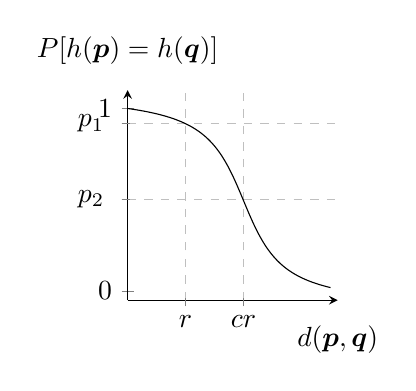
\begin{tikzpicture}
\begin{axis}[
    width=4.25cm,height=4.25cm,
    axis lines=left,
    xlabel={$d(\bm{p},\bm{q})$},ylabel={$P[h(\bm{p})=h(\bm{q})]$},
    every axis y label/.style={at={(current axis.north west)},above=2mm},
    every axis x label/.style={at={(current axis.south east)},below=2mm},
    ymax=1.1,
    ymin=-1.15,
    xmax=8.25,
    ytick={0.9, 0.74, -0.07, -1.05},
    yticklabels={$1$, $p_1\;$, $p_2\;$, $0$ },
    xtick={3, 5},
    xticklabels={ $r$, $cr$ },
    extra x ticks={3, 5},
    extra x tick labels={},
    extra y ticks={0.74, -0.07},
    extra y tick labels={},
    extra tick style={grid=major, dashed},
    ] 
    % \addplot[smooth, tension=0.7] table {\mytable}; 
    \addplot[domain=1:8, smooth, samples=100]
    {0.013*(-atan(x-5)-6.5)};
\end{axis}
\end{tikzpicture}
\end{document}